% Created 2022-01-10 Mon 13:34
% Intended LaTeX compiler: pdflatex
\documentclass[14pt]{article}
\usepackage[utf8]{inputenc}
\usepackage[T1]{fontenc}
\usepackage{graphicx}
\usepackage{grffile}
\usepackage{longtable}
\usepackage{wrapfig}
\usepackage{rotating}
\usepackage[normalem]{ulem}
\usepackage{amsmath}
\usepackage{textcomp}
\usepackage{amssymb}
\usepackage{capt-of}
\usepackage{hyperref}
\usepackage{minted}
\usepackage[a4paper,margin=1in, truedimen]{geometry} \usepackage{graphicx} \usepackage{amssymb}
\usepackage{amsfonts} \usepackage{amsmath}
\author{Max Le}
\date{\today}
\title{Notes on Finite Volume Method MME 9710}
\hypersetup{
 pdfauthor={Max Le},
 pdftitle={Notes on Finite Volume Method MME 9710},
 pdfkeywords={},
 pdfsubject={},
 pdfcreator={Emacs 27.2 (Org mode 9.4.4)}, 
 pdflang={English}}
\begin{document}

\maketitle
\tableofcontents \clearpage


\section{CHAPTER 1: INTRODUCTION}
\label{sec:orgb8e2b9e}
\subsection{Generic Conservation Equation}
\label{sec:orgc302bc7}
Consider the following generic conservation equation:
\begin{equation}
\frac{\partial \phi}{\partial t} + \nabla \cdot (\textbf{u}\phi) + \nabla \cdot \textbf{J}_\phi = S_\phi
\end{equation}
where the variables are defined as:


\begin{center}
\begin{tabular}{ll}
\textbf{Variable} & \textbf{Description}\\
\hline
\(\phi\) & Generic variable\\
\(t\) & Time\\
\textbf{u} & Velocity vector\\
\(\textbf{J}_\phi\) & Diffusive flux of \(\phi\)\\
\(S_\phi\) & Volumetric source/sink of \(\phi\)\\
\hline
\end{tabular}
\end{center}

\subsection{Mass Conservation Equation}
\label{sec:org3a83cb5}
Setting \(\phi = \rho\), where \(\rho\) is the density. Also, mass conservation of a \texttt{continuous} substance does not
have diffusive flux => \(\textbf{J}_\rho = 0\).
\begin{equation}
\frac{\partial \rho}{\partial t} + \nabla \cdot (\textbf{u}\rho) = S_\rho
\end{equation}

\textbf{Notes}:
\begin{itemize}
\item For incompressible, constant density flow:
\begin{itemize}
\item \(\frac{\partial \rho}{\partial t} = 0\)
\item \(\nabla \cdot (\textbf{u}\rho) = \rho \nabla \cdot \textbf{u}\)
\item Result in: \(\nabla \cdot \textbf{u} = \frac{S_\rho}{\rho}\)
\item And if no source/sink => \(\nabla \cdot \textbf{u} = 0\)
\end{itemize}
\end{itemize}

\subsection{Momentum Conservation Equation}
\label{sec:org4809a81}
Setting \(\phi = \rho \textbf{u}\). Diffusive flux term \(\textbf{J}_\textbf{u} = -\nabla \cdot \sigma\), where
\(\sigma\) is the fluid stress tensor. 

\begin{equation}
\frac{\partial (\rho \textbf{u})}{\partial t} + \nabla \cdot (\rho \textbf{uu})  = \nabla \cdot \sigma +
S_\textbf{u}
\end{equation}
The stress tensor, \(\sigma\) can be expressed in terms of pressure (\(p\)) and viscous stress tensor (\(\tau\))
and identity matrix, \(I\):

\begin{equation}
\sigma = -p\textbf{I} + \tau
\end{equation}
After substituting, we get the following form of the momentum conservation equation:
\begin{equation}
\frac{\partial (\rho \textbf{u})}{\partial t} + \nabla \cdot (\rho \textbf{uu})  = -\nabla p + \nabla \cdot \tau
+ S_\textbf{u}
\end{equation}
For incompressible Newtonian fluid, we can rewrite \(\tau\) in terms of the dynamic viscosity, \(\mu\)
\(\tau = \mu(\nabla \textbf{u}+\nabla \textbf{u}^T)\).  Thus, a momentum conservation equation for \uline{incompressible},
\uline{Newtonian} fluid, \uline{constant velocity}:

\begin{equation}
\frac{\partial (\rho \textbf{u})}{\partial t} + \nabla \cdot (\rho \textbf{uu})  = -\nabla p + \mu \nabla^2
\textbf{u} + S_\textbf{u}
\end{equation}

\subsection{Energy Conservation Equation}
\label{sec:orgce7e730}
Setting \(\phi = \rho h\) with \(h\) being the specific enthalpy of a substance at a given state. Thus, the unit for \(\phi\) is
energy per unit volume. The diffusive flux is given by Fourier's law: \(J = -k \nabla \textbf{T}\) with \(k\) is the thermal conductivity.
\begin{equation}
\frac{\partial (\rho h)}{\partial t} + \nabla \cdot (\rho \textbf{u} h)  = \nabla \cdot (k \nabla \textbf{T}) +
S_h
\end{equation}

If we assume:
\begin{itemize}
\item incompressible flow
\item constant specific heat capacity, \(h = c_p \textbf{T}\)
\item constant thermophysical properties (\(k\) and \(\rho\))
\item no source term
\end{itemize}

\begin{equation}
\frac{\partial (\textbf{T})}{\partial t} + \nabla \cdot (\textbf{u T})  = \alpha \nabla ^2 \textbf{T}
\end{equation}

where \(\alpha = \frac{k}{\rho c_p}\) is the thermal diffusivity. 

\subsection{Discretization of the Generic Conservation Equation}
\label{sec:org5dd5f85}
Our generic variable, \(\phi\) is a function of of spatial and time: \(\phi = \phi (\textbf{x},t)\), where
\(\textbf{x} = (x,y,z)\). Note that spatial variable can be influenced "\textsubscript{one} way\_" or "\textsubscript{two} way\_", i.e.
\begin{itemize}
\item One way: changes in \(\phi\) only occur due to change on one side of that location
\item Two way: changes in \(\phi\) occur due to changes on both side of that location.
\end{itemize}
For example, heat conduction in the image below at cell \(i\) is influenced by cell \(i-1\) and
\(i+1\). Here, \(\textbf{x}\) is a \uline{two way} coordinate for heat conduction

\begin{center}
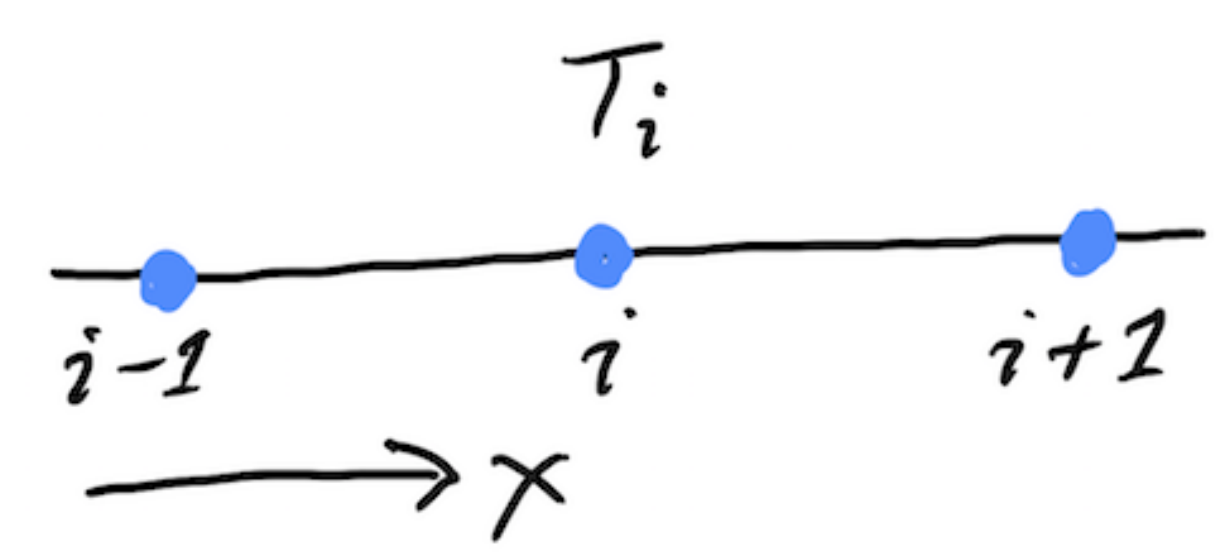
\includegraphics[scale=0.2]{pic/heatTwoway.png}
\end{center}
Now consider transient heat convection/conduction. The temperature at any given time is influenced by
existing conditions before that point \textbf{in time}. Here, \(\textbf{t}\) is a \uline{one way} coordinate for transient heat conduction/convection

\begin{center}
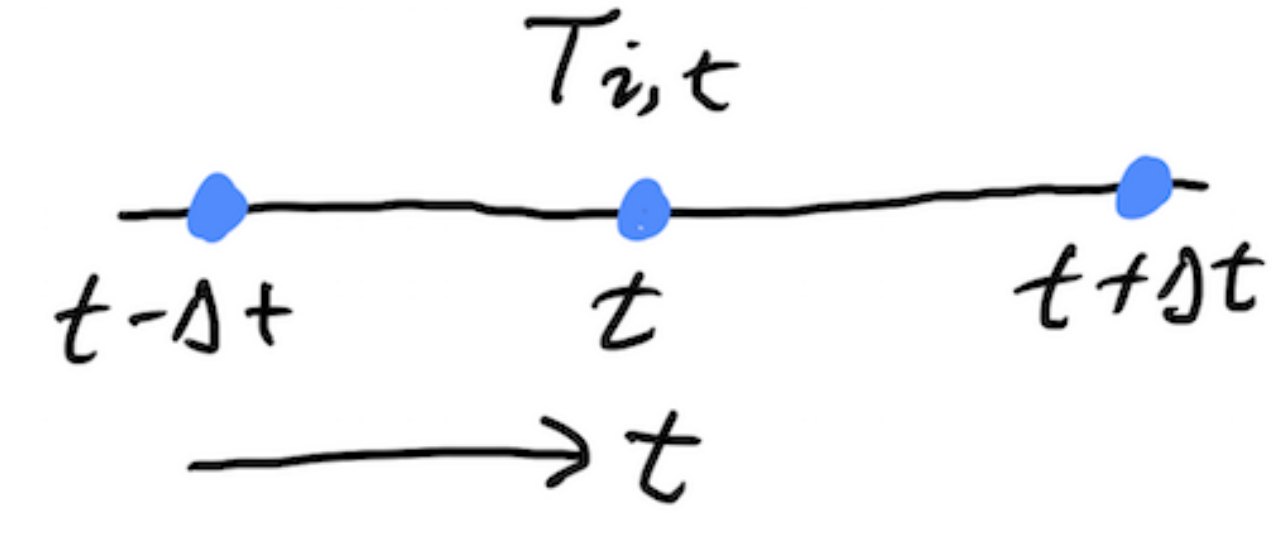
\includegraphics[scale=0.2]{pic/heatOneway.png}
\end{center}
Recall our generic conservation equation:
\begin{equation*}
\frac{\partial \phi}{\partial t} + \nabla \cdot (\textbf{u}\phi) + \nabla \cdot \textbf{J}_\phi = S_\phi
\end{equation*}
We consider the diffusion term or \textbf{elliptic PDE} :  \(\boxed{\nabla \cdot \textbf{J}_\phi}\) to be \uline{two-way in space}\\
Likewise, the convection term or \textbf{parabolic PDE} :  \(\boxed{\nabla \cdot (\textbf{u}\phi)}\) to be \uline{one-way in space} 

\subsection{Main idea behind Discretization}
\label{sec:org08c2ec0}
Our goal is to:
\begin{itemize}
\item replace the PDEs' continuous solution with \uline{discrete} solution, at \uline{specific location} that approximates the continuous
solution suitably.
\end{itemize}
For finite volume:
\begin{enumerate}
\item domain is split into \uline{non overlapping finite} regions that fill the domain
\item the discrete point is at the \uline{centroid} of each control volume with volume \(V_p\), at position \(\textbf{x}_p\)
\item surround these cells, we have the "faces". At the center of these "faces", we have the integration point at position
\(\textbf{x}_{ip}\)
\item the governing equations are then integrated over a control volume, where surface flux terms and volume source terms are
balanced. 
\begin{center}
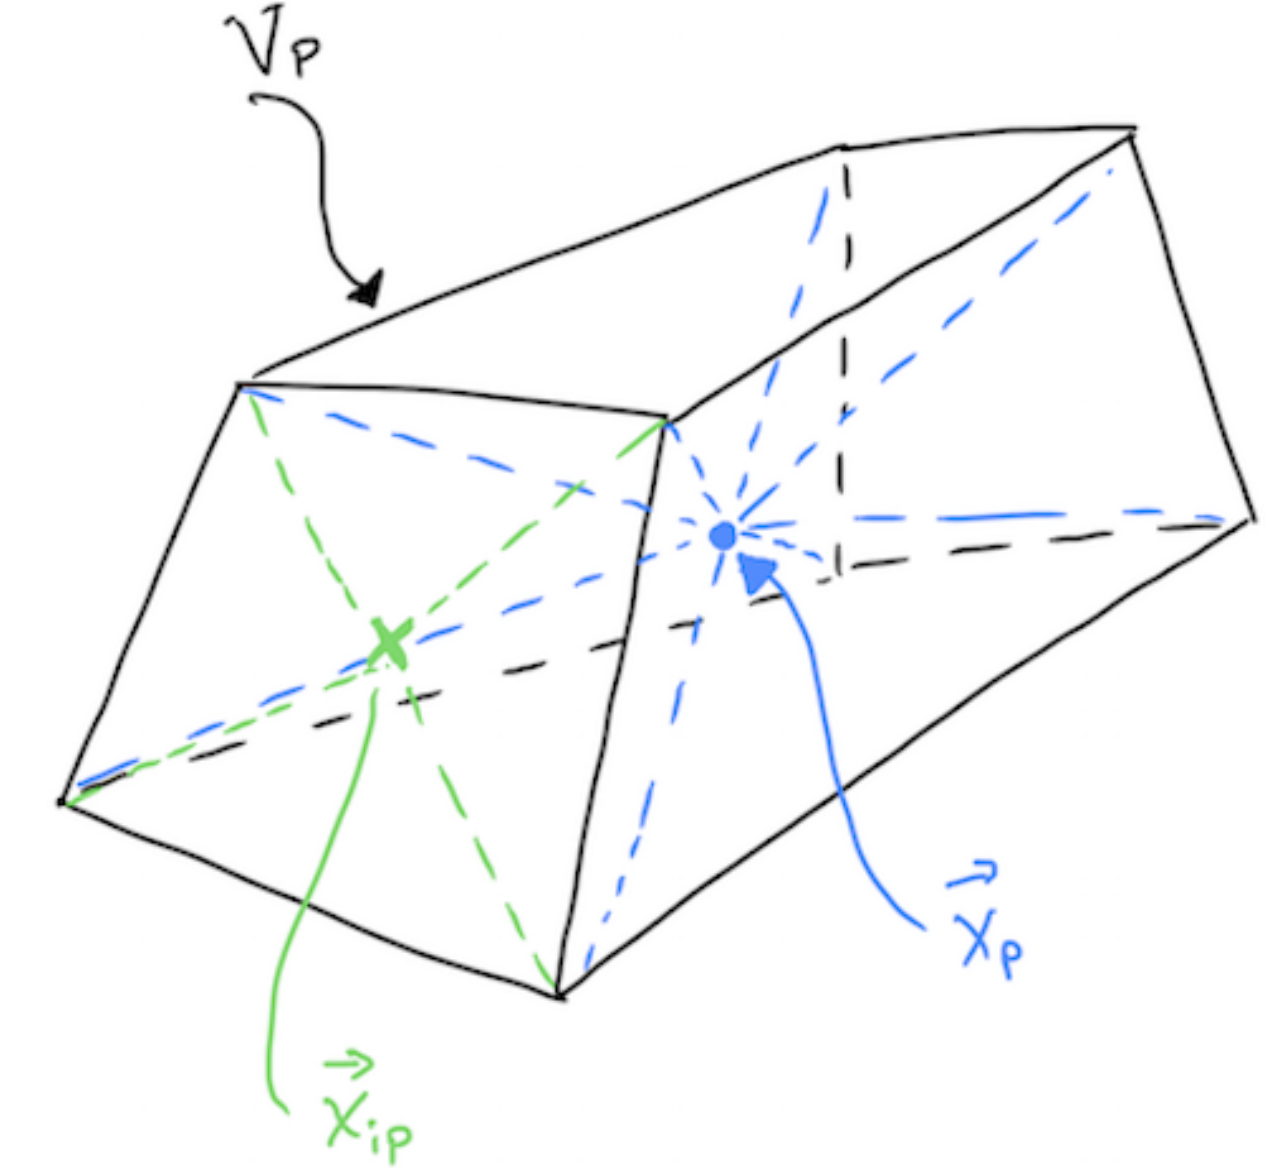
\includegraphics[scale=0.2]{pic/finiteVolumeElement.png}
\end{center}
\end{enumerate}
\subsection{Determine Cell Centre + Face Integration Points}
\label{sec:orgbb80a07}
\uline{Cell centre} => location of \uline{solution} variables.\\
Points on \uline{face} => \uline{fluxes} are evaluated.\\
Consider a volume integral of a quantity \(\phi\), we may express this integral in discrete form as follow:
\begin{equation}
\int_V \phi dV \approx \phi_P V_P 
\end{equation}
where \(\phi_P\) is the value of \(\phi\) at some internal within \(V\) and \(V_P\) is total volume of the cell:
\begin{equation}
V_P = \int_V dV 
\end{equation}
To prove the above result, we expand \(\phi\) in a Taylor series about the point \(P\).
\begin{equation}
\phi \approx \phi_P + \nabla \phi_P (\textbf{x} - \textbf{x}_P) + \nabla^2 \phi_P (\textbf{x}-\textbf{x}_P)(\textbf{x}-\textbf{x}_P) + .... O(\delta^3) 
\end{equation}
with \(\delta\) being the characteristic grid spacing. Substitute this into our assumed expression for \(V_P\):
\begin{equation}
\int_V \phi dV \approx \int_V [\phi_P + \nabla \phi_P (\textbf{x} - \textbf{x}_P) + \nabla^2 \phi_P (\textbf{x}-\textbf{x}_P)(\textbf{x}-\textbf{x}_P) + .... O(\delta^3)]dV 
\end{equation}
We note that \(\phi_P\) and its derivatives are constants:
\begin{equation}
\int_V \phi dV \approx \phi_P dV + \nabla \phi_P \int_V (\textbf{x}-\textbf{x}_P) dV + \nabla^2 \phi_P \int_V (\textbf{x}-\textbf{x}_P)(\textbf{x}-\textbf{x}_P)dV + .... O(\delta^3) 
\end{equation}
Because our \(\textbf{x}_P\) point is at centroid, so \(\int_V (\textbf{x}-\textbf{x}_P) dV = 0\). Likewise, the last term is also neglected,
resulting in:
\begin{equation}
\int_V \phi dV \approx [\phi_V + O(\delta^2)]V_P
\end{equation}
This means that there is a second order error when approximating the cell volume in this way.  This is OK because the accuracy of
the method is also second order.\\
\textbf{Note}: If our \$\textbf{x}\textsubscript{P}\} does not lie at the centroid of the cell. The second term,\(\int_V (\textbf{x}-\textbf{x}_P) dV\) does not go
to zero, making our approximation to be 1st order, which is worse. 
\subsection{Transient term}
\label{sec:org896df99}
Here we deal with the transient term, \(\frac{\partial \phi}{t}\). Discretization of this term relies on:
\begin{itemize}
\item order of accuracy
\item implicit vs explicit
\end{itemize}
The idea is to integrate this term over control volume \(V_P\) and some time step \(\Delta t = t_1 - t_0\) to get
the formula for the discretization.
\begin{equation}
\int_{t_0}^{t_1} \int_V \frac{\partial \phi}{\partial t}dVdt \approx (\phi V_P)^{t_1} - (\phi V_P)^{t_0} 
\end{equation}
\subsection{Advection term}
\label{sec:org4b3b3fa}
Here we deal with the advection term, \(\nabla \cdot (\textbf{u} \phi)\). Similar to the transient term, the formula for the
discretization can be obtained by integrating over the control volume \(V_P\). We also employ Gauss' theorem to convert
\uline{volume integral} to \uline{surface integral}:
\begin{equation}
\int_V \nabla \cdot (\textbf{u}\phi)dV = \int_S (\textbf{u}\phi) \cdot \textbf{n}dS
\end{equation}
For the surface integral, we approximate by summing up over the faces surrounding the cell, each with area \(A_{ip}\).
\begin{equation}
\int_S (\textbf{u}\phi) \cdot \textbf{n}_{ip}dS \approx \sum_{i=0}^{N_{ip}-1} \textbf{u}_{ip} \cdot \textbf{n}_{ip} \phi_{ip}A_{ip}
\end{equation}
\textbf{Note}:
\begin{itemize}
\item using C program notation, so we sum from 0 till \(N_{ip}-1\)
\item approximate \(\textbf{u}_{ip}\) by many interpolation methods
\item interpolating \(\phi_{ip}\) carefully to obtain \uline{stable} numerical method.
\end{itemize}
\subsection{Diffusion term}
\label{sec:org2098a58}
Now, we deal with the diffusion term, \(\nabla \cdot \textbf{J}_\phi\). Similar to the advection term, we integrate over a control
volume, then apply Gauss' theorem
\begin{equation}
\int_V \nabla \cdot \textbf{J}_\phi dV = \int_S \textbf{J}_\phi \cdot \textbf{n}dS
\end{equation}
Again, the surface integral is approximated as discrete sum over the faces surrounding the cell:
\begin{equation}
\int_S \textbf{J}_\phi \cdot \textbf{n}dS \approx \sum_{i=0}^{N_{ip}-1} \textbf{J}_{\phi, ip} \cdot \textbf{n}_{ip}\textbf{A}_{ip}
\end{equation}
where the flux, \(\textbf{J}_{\phi,ip}\) is interpolated from neighboring cell values. 
\subsection{Source term}
\label{sec:org2f983f7}
Recall our source term: \(S_\phi\), we assume that the source term is \uline{piecewise continuous}, with one specific value, \(S_\phi\),
being represented by each cell. We can then write:
\begin{equation}
\int_V S_\phi dV \approx S_\phi V_P
\end{equation}
Generally, the source term may depend on \(\phi\) so linearization is needed to obtain \uline{stable} numerical method. 
\subsection{Linearization}
\label{sec:org49b8697}
With regard to our last point about \(J_\phi\), the discretized terms depend non linearly on the solution. This non-linearity
is caused by:
\begin{itemize}
\item source term depend non linearly on primitive variable, e.g. \(J_\phi\).
\item non linearities in the governing equation, e.g. advection term \(\nabla \cdot (\textbf{u} \phi)\)
\item on non-orthogonal grid, gradient correction terms are needed <= these are non linear.
\end{itemize}
To linearize, we assume the governing PDE is represented by the following general differential operator
\begin{equation}
L(\phi^*) = 0
\end{equation}
where:\\
\begin{itemize}
\item \(\phi^*\) = the continuous solution to the PDE
\item Note that to solve a PDE using finite volume, the continuous solution \(\phi^*\) is approximated by the discrete solution vector
\(\phi \in \mathbb{R}\) on \(N\) number of control volume. Our PDE is then integrated over each control volume and each term in the
governing equation is approximated using the discrete solution \(\phi\)
\item Of course, the numerical solution will not satisfy the discretized equation exactly; rather we will have a residual,
\(\textbf{r} \in \mathbb{R}^N\).
\end{itemize}
We expand the residual about the solution \(\phi_i\) at iteration \(i\), and find the solution where \(r = 0\):
\begin{equation}
\textbf{r}(\phi_i) + \left. \frac{\partial \textbf{r}}{\partial \phi}\right|_{\phi_i}(\phi - \phi_i) = 0
\end{equation}
We define the \textbf{Jacobian of the residual vector} as:
\begin{equation}
\textbf{J}(\phi) = \frac{\partial \textbf{r}}{\partial \phi}
\end{equation}
We use this to update according to fix point iteration:
\begin{equation}
\phi = \phi_i + \Delta \phi_i
\end{equation}
where:
\begin{equation}
\Delta \phi = (\phi - \phi_i)
\end{equation}
and:
\begin{equation}
\textbf{J}(\phi_i)\Delta \phi = -\textbf{r}(\phi_i)
\end{equation}
The remaining unknowns are: the residual vector \(\textbf{r}\) and Jacobian matrix \(\textbf{J}(\phi_i)\).\\
\textbf{Note}: we can express the linear system for a control volume P as:
\begin{equation}
a_P\delta \phi_P + \sum_{nb} a_{nb}\delta \phi_{nb} = -r_P
\end{equation}
where \(nb\) is sum over all neighboring cells.  The coefficients are defined as:
\begin{align}
a_P &= \frac{\partial r_P}{\partial \phi_P}\\
a_{nb} &= \frac{\partial r_P}{\partial \phi_{nb}}
\end{align}

\clearpage
\section{CHAPTER 2: STEADY DIFFUSION EQUATION}
\label{sec:org632af7a}
\subsection{Problem Definition}
\label{sec:orgf9ca466}
We consider the solution of a \uline{steady}, \uline{1D} heat diffusion equation
\begin{equation}
-k \nabla^2 T - S = 0
\end{equation}
\subsection{Discretization}
\label{sec:org264146a}
Recall our diffusion term can be discretized as:
\begin{equation}
\int_S \textbf{J} \cdot \textbf{n} dS \approx \sum_{i=0}^{N_{ip}-1} \textbf{J}_{ip}\cdot \textbf{n}_{ip}A_{ip}
\end{equation}
Our flux \(\textbf{J}\) here is the \uline{diffusive} flux, so: \(\textbf{J} = -k \nabla T\). Thus:
\begin{equation}
\int_S \textbf{J} \cdot \textbf{n} dS \approx -\sum_{i=0}^{N_{ip}-1} k_{ip} \nabla T_{ip}  \cdot \textbf{n}_{ip}A_{ip}
\end{equation}
We assume constant thermal conductivity, \(k_{ip} = k\). A 1D control volume, with West/East faces and unit vectors drawn, is shown below:
\begin{center}
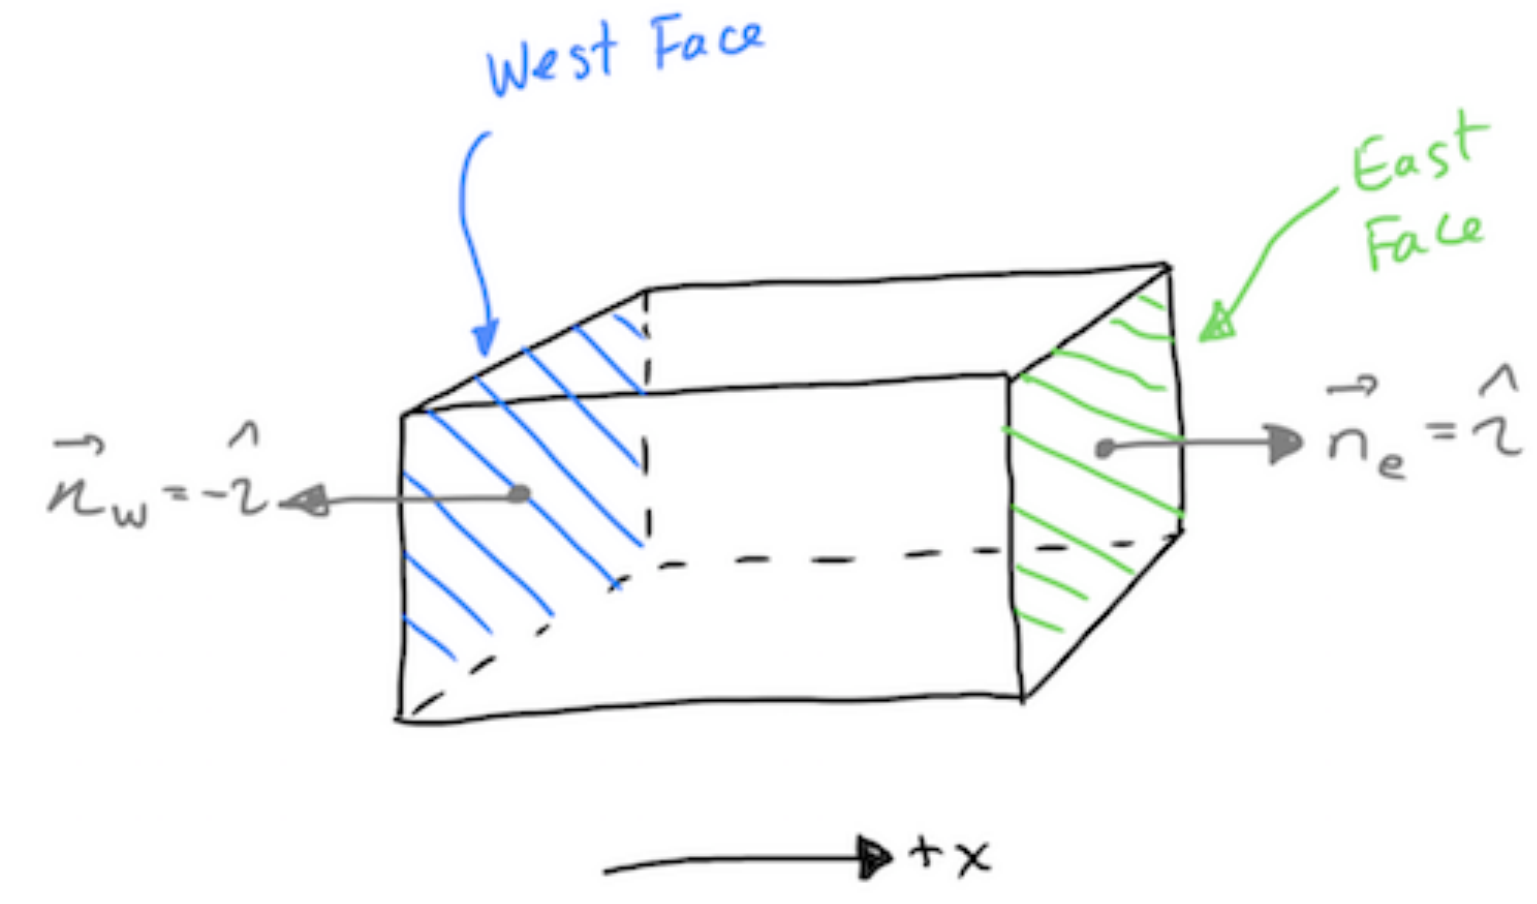
\includegraphics[scale=0.2]{pic/heat1D_CV.png}
\end{center}
Since we are in 1D, our unit vector is in the \(\textbf{i}\) only.\\
Thus, \(\nabla T \cdot \textbf{n} = \nabla T \cdot \textbf{i}\).\\
But, \(\nabla T \cdot \textbf{i} = \left < \frac{\partial T}{\partial x} \textbf{i} + \frac{\partial T}{\partial y} \textbf{j} + \frac{\partial T}{\partial z} \textbf{k}
  \right > \cdot \left <1 \textbf{i} + 0 \textbf{j} + 0 \textbf{k}    \right> = \frac{\partial T}{\partial x}\). \\
With these points in mind, the discretization for the diffusion term is simplified to:
\begin{equation}
\int_S \textbf{J} \cdot \textbf{n} dS \approx k \left .\frac{\partial T}{\partial x}\right|_w A_w
- k \left .\frac{\partial T}{\partial x}\right|_e A_e 
\end{equation}
The diagram below shows the cell locations and the nomenclature for the distance between them, note how \(\Delta x\) is center-center
\begin{center}
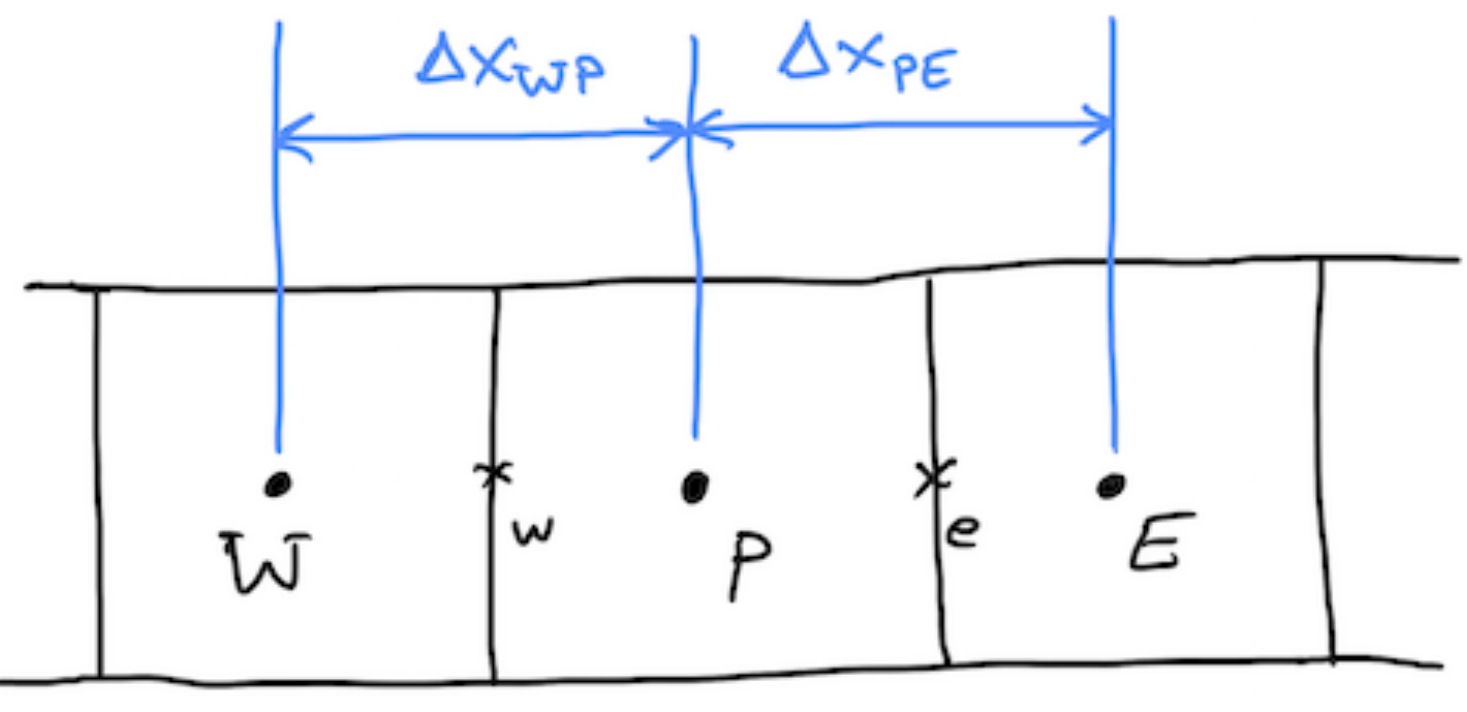
\includegraphics[scale=0.2]{pic/heat1D_cell.png}
\end{center}
We apply \uline{finite differences} to the derivatives in the diffusion term, i.e.:
\begin{equation}
k \left .\frac{\partial T}{\partial x}\right|_w A_w - k \left .\frac{\partial T}{\partial x}\right|_e A_e
= k\frac{T_P-T_W}{\Delta x_{WP}}A_w - k\frac{T_E-T_P}{\Delta x_{PE}}A_e
\end{equation}
Our discretized source term is simply:
\begin{equation}
\int_V SdV \approx S_PV_P
\end{equation}
where \(S_P\) = value of source term \textbf{within} the cell, and \(V_P\) = cell volume.\\
Put everything on one side, we can form the \uline{residual equation} for the cell \(\textbf{P}\) as:
\begin{equation}
r_P = - k\frac{T_E-T_P}{\Delta x_{PE}}A_e + k\frac{T_P-T_W}{\Delta x_{WP}}A_w - S_PV_P
\end{equation}
or expressing in terms of the diffusive fluxes, \(\textbf{F}^d\), through each face:
\begin{equation}
r_P = F_{e}^d - F_{w}^d - S_PV_P
\end{equation}
where:\\
\begin{alignat}{2}
F_{e}^d &= - k\frac{T_E-T_P}{\Delta x_{PE}}A_e &&= -D_e(T_E- T_P)\\
F_{w}^d &= - k\frac{T_P-T_W}{\Delta x_{WP}}A_w &&= -D_w(T_P- T_W)\\
D_e &= \frac{kA_e}{\Delta x_{PE}}\\
D_w &= \frac{kA_w}{\Delta x_{WP}}
\end{alignat}
Our cell residual equation is then:
\begin{equation}
r_P = D_w (T_P-T_W)-D_e(T_E-T_P)-S_PV_P
\end{equation}
The linearized coefficients are then calculated as:
\begin{align}
a_P &= \frac{\partial r_P}{\partial T_P} = D_w + D_e - \frac{\partial S_P}{\partial T_P}V_P\\
a_W &= \frac{\partial r_P}{\partial T_W} = -D_w\\
a_E &= \frac{\partial r_P}{\partial T_E} = -D_e
\end{align}
Recall that we can form an algebraic system of equation for each control volume like this:
\begin{align}
a_P\delta \phi_P + \sum_{nb} a_{nb}\delta \phi_{nb} &= -r_P\\
a_P\delta T_P + a_W\delta T_W + a_E \delta T_E &= -r_P 
\end{align}
The above linear system of equations can be written as as tridiagonal matrix, like this:
\begin{center}
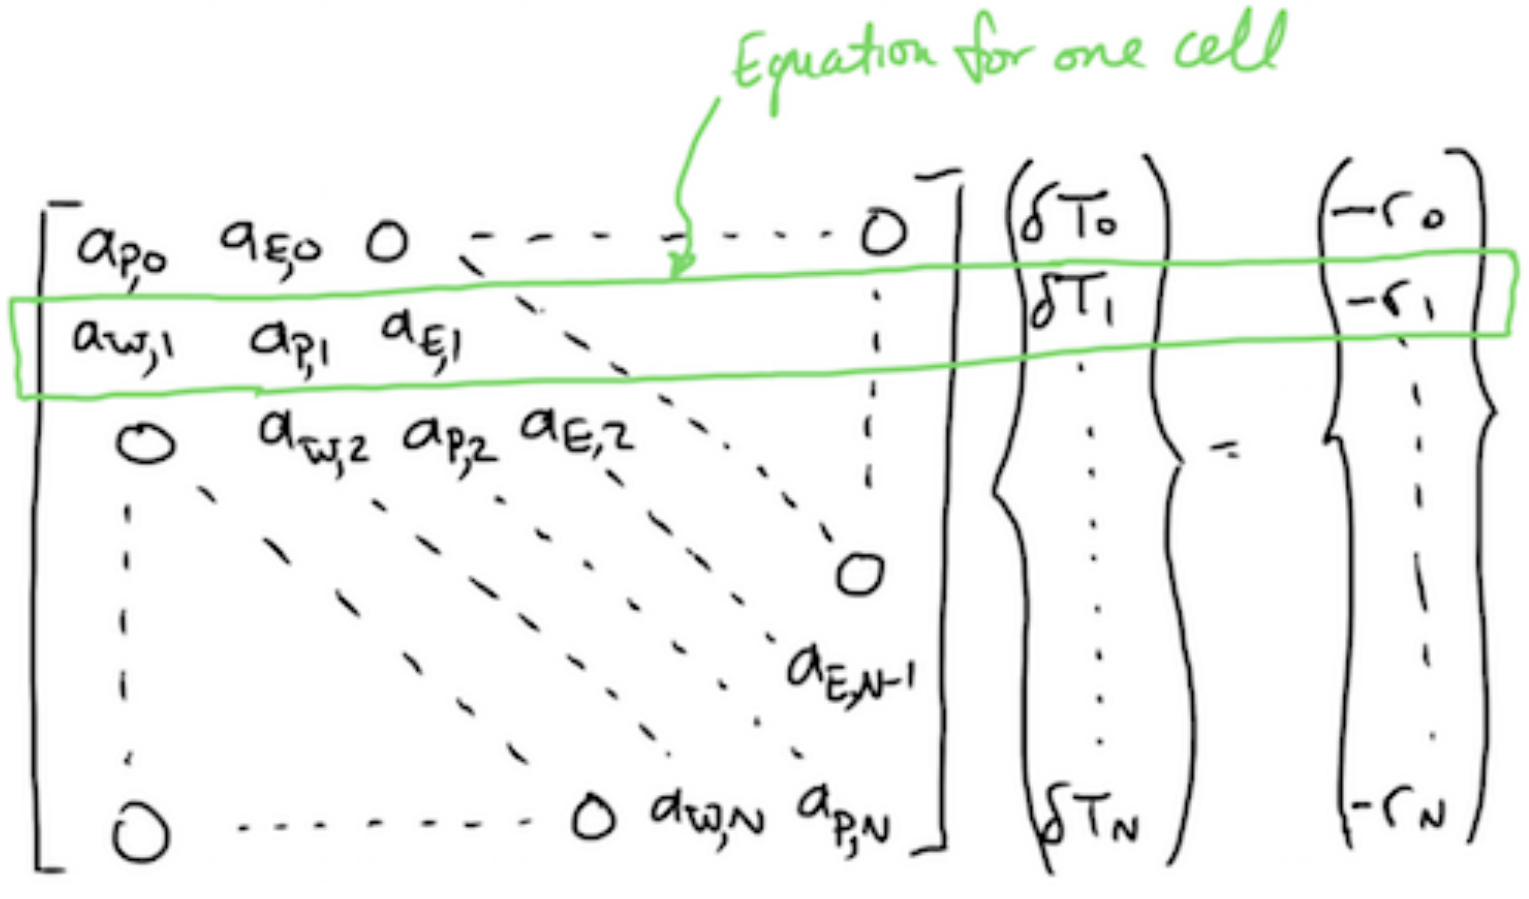
\includegraphics[scale=0.2]{pic/heat1D_tridiagonal.png}
\end{center}
\textbf{Note}: The first and last row only has 2 non zero elements each. This is because these are the left most/right most side and they are
adjacent to the domain boundary. Therefore, special \uline{boundary conditions} are needed to be set. \\
In matrix notation, we are solving:
\begin{equation}
\textbf{A}\textbf{x} = \textbf{b}  
\end{equation}
where \(\textbf{A}\) is the Jacobian matrix, \(\textbf{b} = \textbf{-r}\) is the residual vector, \(\textbf{x} = \delta \textbf{T}\)
is the solution correction. At each current iteration \(i\), the solution is updated according to:
\begin{equation}
\textbf{T} = \textbf{T}_i + \delta \textbf{T}i
\end{equation}
\subsection{Source Terms}
\label{sec:orgb67f0b8}
Our source term can have many forms, depending on the type of heat source. We will assume \emph{external convection}
and \emph{radiation exchange}:
\begin{itemize}
\item For external convection:
\begin{equation}
\frac{S_{conv,P}}{V_P} = -hA_0(T_P-T_{\infty,c})
\end{equation}
where:
\begin{itemize}
\item \(h\) is the convective coefficient.
\item \(A_0\) is external surface area of the cell \(P\).
\item \(T_P\) is temperature at the centroid of cell \(P\).
\item \(T_{\infty,c}\) is the ambient temperature for the convection process.
\end{itemize}
\item For radiation exchange:
\begin{equation}
\frac{S_{rad}}{V_P} = -\epsilon \sigma A_0(T_P^4 - T_{\infty,r}^4)
\end{equation}
where:
\begin{itemize}
\item \(\epsilon\) is the surface emissivity.
\item \(\sigma\) is the Stefan-Boltzmann constant.
\item \(T_{\infty,r}\) is the surrounding temperature for radiation exchange.
\end{itemize}
\end{itemize}
\subsection{Discussion of Discretization Procedure}
\label{sec:org9cd07c7}
\subsubsection{Temperature Profile Assumptions}
\label{sec:orgd82e862}
When computing the diffusive fluxes through the faces, we assumed a \textbf{piecewise-linear profile} for the temperature.
This ensures that the derivatives are defined at the integration points and provides consistency for flux
at control-volume faces. For the source term, \textbf{piece-wise constant profile} is used, implying a single value of the source
term in each cell. Note that for piece-wise constant profile, the derivatives are not defined at integration points, due to
jump discontinuity. So if fluxes will be inconsistent if piecewise-constant profile is used for temperature.
\begin{center}
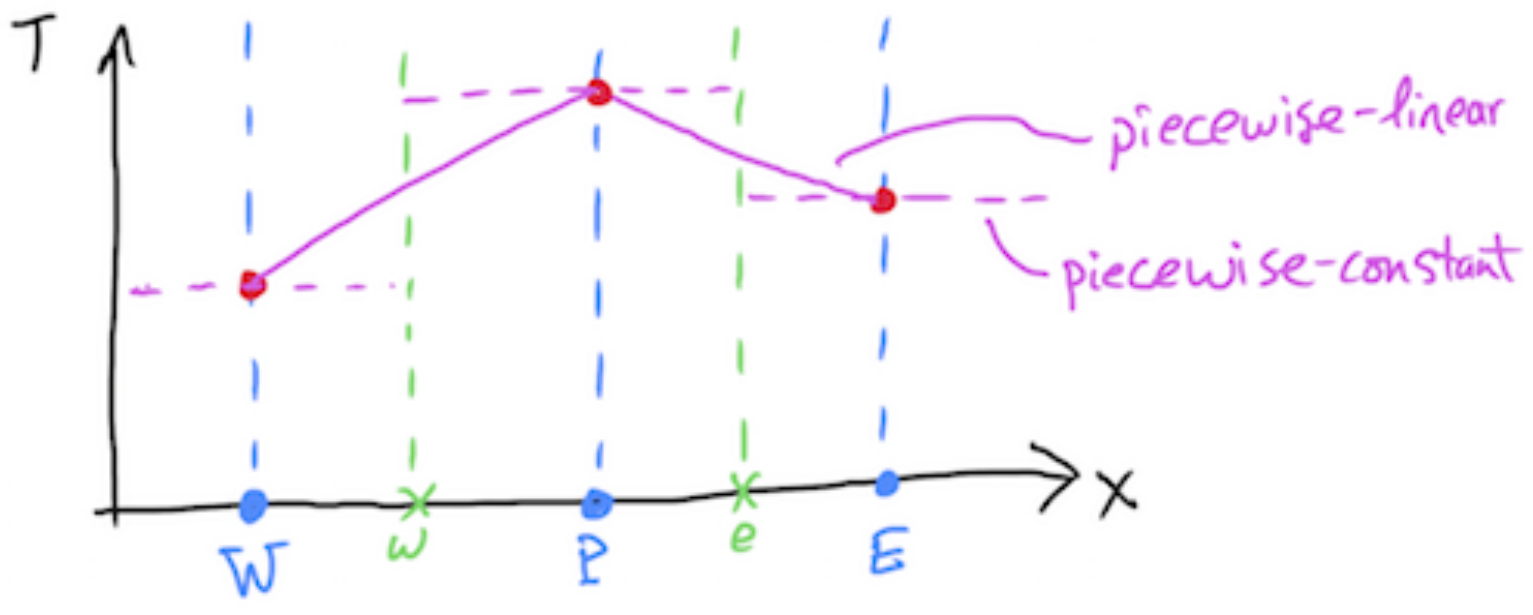
\includegraphics[scale=0.2]{pic/heat1D_profilePW.png}
\end{center}
\subsubsection{Implementation of Linearization}
\label{sec:org79383e5}
In Patakar's method, the solution of the linear system \textbf{is} the solution for the variables at the control volume center.\\
In our method, the solution of the linear system is the \textbf{correction} to apply to the previous iteration of the solution. \\
The correction method is preferred because:
\begin{itemize}
\item at convergence, the solution for the correction goes to zero \(\rightarrow\) zero a good initial guess for the linear solver.
\item linear system involves the residual vector. In Patankar's, there are more work to calculate the residual vector.
\end{itemize}
\subsubsection{Properties of the Discrete Algebraic Equations}
\label{sec:orgb2c042e}
Recall our algebraic equation for the linear system
\begin{equation}
a_P\delta T_P + a_W\delta T_W + a_E \delta T_E = -r_P 
\end{equation}
In Rule 2, we require that \(a_P > 0\) and \(a_W, a_E < 0\). The reason for this is if we consider the case with no source,
and the solution converge, \(r_P \rightarrow 0\):
\begin{equation}
a_P\delta T_P = -a_W\delta T_W - a_E \delta T_E  
\end{equation}
Now, suppose both \(T_P\) and \(T_E\) are pertubed.  If either of these temperatures were to rise, then \(T_P\) would also rise.
Similarly, if either temperatures were to drop, \(T_P\) should also drop. Therefore, to ensure correct physical effect, if
\(a_P > 0\) then \(a_W, a_E > 0\).\\
Consider the two cells (\(P\) and \(E\)) below:
\begin{center}
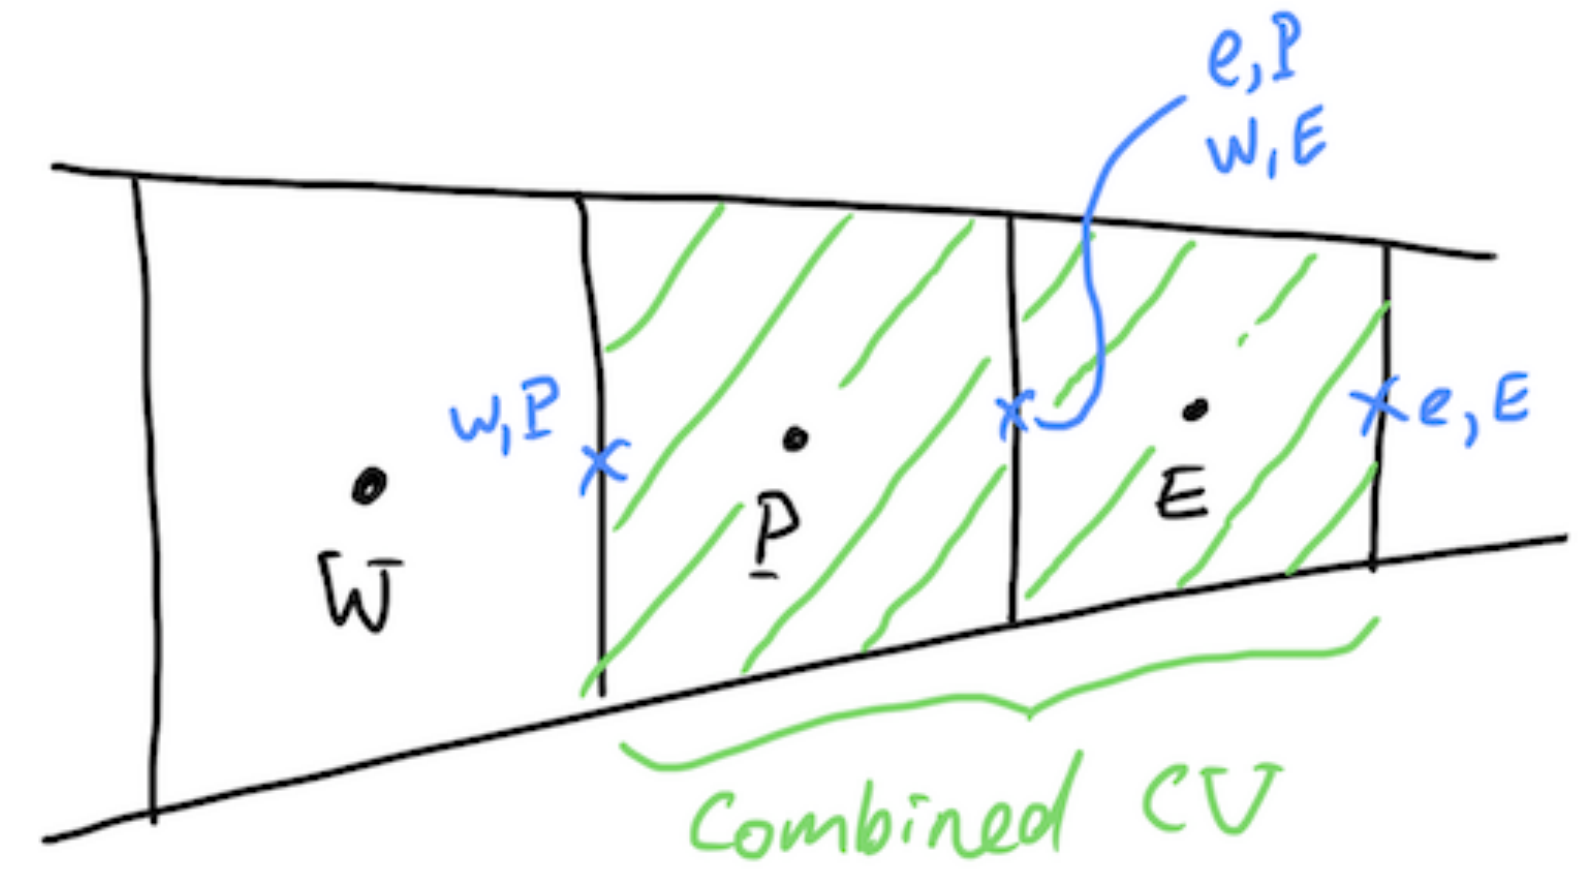
\includegraphics[scale=0.2]{pic/heat1D_cell_combined.png}
\end{center}
At convergence, \(r_P = 0\), the equation for the control volume \(P\) is:
\begin{equation}
F_{e,P}^d - F_{w,P}^d - S_PV_P = 0
\end{equation}
For the control volume \(E\):
\begin{equation}
F_{e,E}^d - F_{w,E}^d - S_EV_E = 0
\end{equation}
Adding these equations together gives:
\begin{equation}
F_{e,P}^d - F_{w,P}^d +  F_{e,E}^d - F_{w,E}^d- S_PV_P - S_EV_E = 0
\end{equation}
Note that \(F_{e,P}^d = F_{w,E}^d\) by continuity, i.e. the flux at cell \(P\) going eastward should be the same flux going
from westward at cell \(E\). If these are not equal, then it implies that there is a fictuous force at the face, which is
not reasonable. Therefore, our algebraic equation for control volume \(P\) and \(E\) becomes:
\begin{equation}
 F_{e,E}^d - F_{w,P}^d - S_PV_P - S_EV_E = 0
\end{equation}
The above equation demonstrates integral conservation: a balance of the total source term within the combined control volume with
the net diffusive flux from that same control volume. In addition, recall the definition of the diffusive flux:
\begin{align}
F_{e,P}^d &= -k \frac{T_E-T_P}{\Delta x_{PE}} A_{e,P}\\
F_{w,E}^d &= -k \frac{T_E-T_P}{\Delta x_{PE}} A_{w,E}
\end{align}
From the gemeotry of the grid, \(A_{e,P} = A_{w,E}\); therefore, it is in fact the two-point finite difference estimation of the
derivative that cause the fluxes to be equal. This is also due to the piecewise-linear profile that we assume. If we assume a
\textbf{parabolic profile} instead, there is no guarantee that the fluxes would be equal. Instead, we would have:
\begin{align}
F_{e,P}^d &= f(T_W, T_P, T_E)\\
F_{w,E}^d &= f(T_P, T_E, T_{EE})
\end{align}
This means that the flux through the common face depends on different temperature, so we cannot be sure that the derivative from either
side is consistent. 
\begin{center}
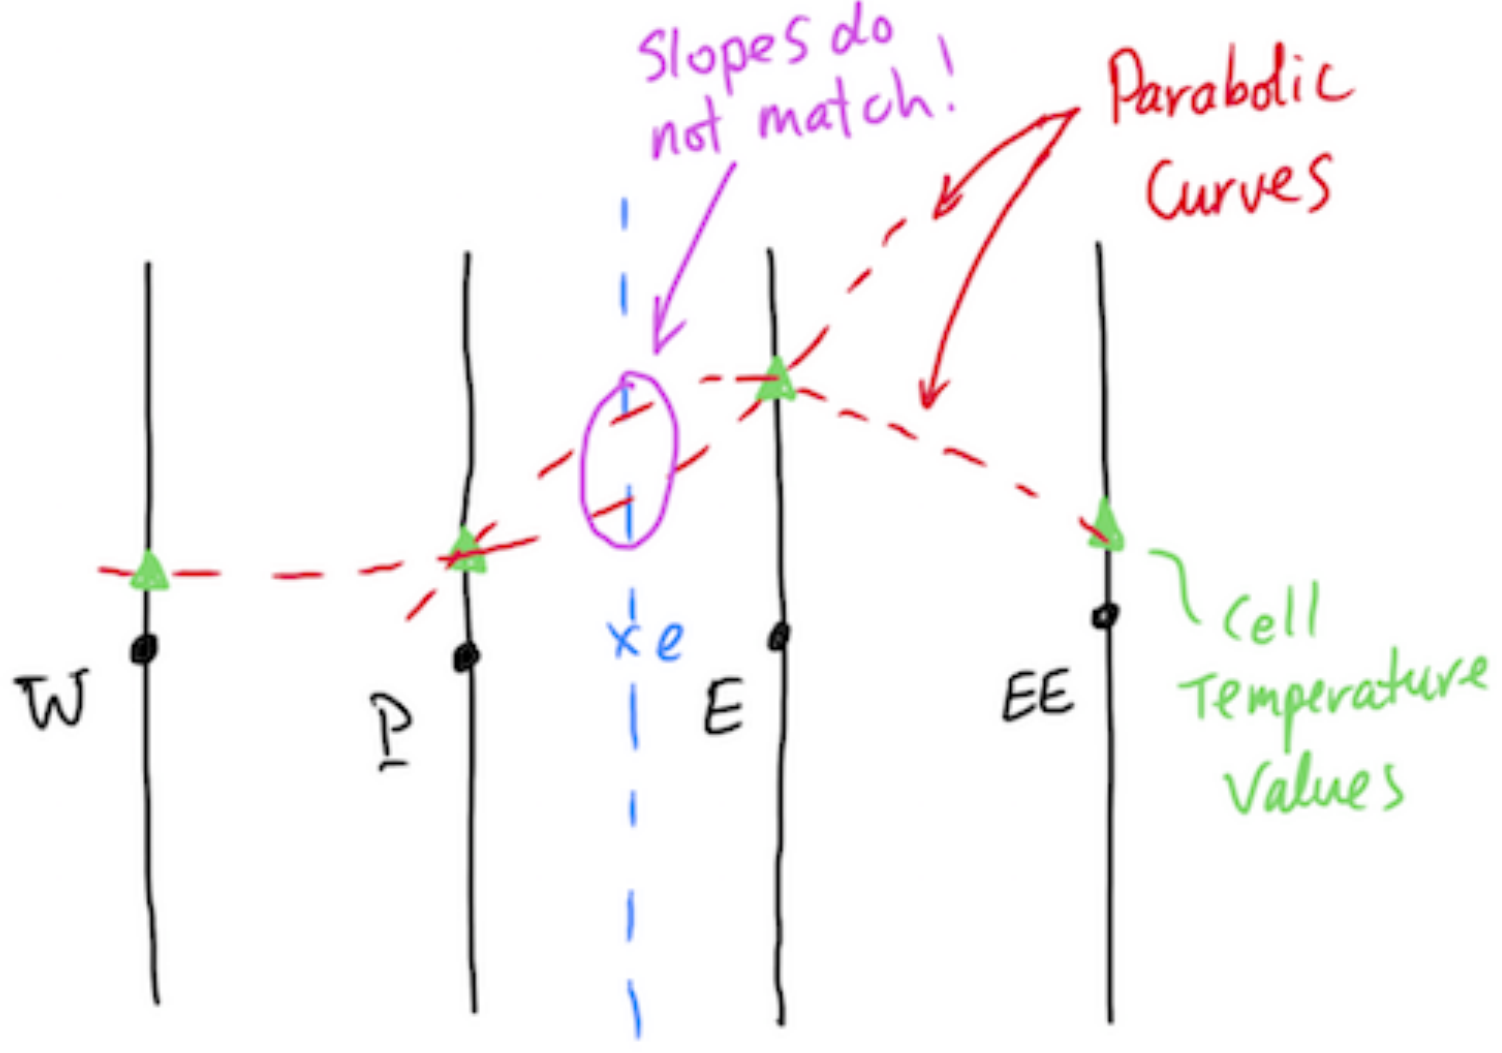
\includegraphics[scale=0.2]{pic/heat1D_profilePARABOLIC.png}
\end{center}
\subsubsection{Implemenation: \href{1D\_heat\_diffusion.py}{Python code}}
\label{sec:org2316d15}
\clearpage
\section{CHAPTER 3: TRANSIENT 1D HEAT DIFFUSION}
\label{sec:orge5e118f}
\subsection{Problem Definition}
\label{sec:org6b4b2eb}
In contrast to the steady case, here we are solving the following transient 1D heat diffusion equation
\begin{equation}
\frac{\partial (\rho c_p T)}{\partial t} = k \nabla^2 T + S
\end{equation}
assuming constant \(\rho\) and \(c_p\)
\subsection{Discretization}
\label{sec:org9c62bcb}
Integrating the governing equation through space and time yields:
\begin{equation}
\int_{t_0}^{t_1} \int_{V} \frac{(\partial \rho c_p T)}{\partial t} dt dV = \int_{t_0}^{t_1} \int_{V} k \nabla^2 T dt dV + \int_{t_0}^{t_1} \int_{V} S dt dV
\end{equation}
By assuming a timestep \(\Delta t = t_1 - t_0\), we also assume that the solution is stored at time levels \(t\) and later at \(t + \Delta t\). Thus, we can assume various profiles for the integrands as functions of time.  Here, we will examine the following:
\begin{itemize}
\item \textbf{Fully explicit}: evaluate the integrands on RHS at initial time level, \(t_0 = t\).
\item \textbf{Fully implicit}: evaluate the integrands on RHS at final time level, \(t_1 = t_0 + \Delta t\)
\item \textbf{Crank Nicolson}: assume a linear profile of the RHS over the interval \(\Delta t\).
\end{itemize}
For the LHS, we interchange the order of integration, which results in this, for a control volume \(\textbf{P}\):
\begin{equation}
\int_{t_0}^{t_1} \int_{V} \frac{(\partial \rho c_p T)}{\partial t} dt dV = (\rho c_p T_p)^{t+\Delta t} - (\rho c_p T_p)^t 
\end{equation}
Recall that for the steady case, the diffusive term is the difference in flux. Here, we add a weighting function \(w\) to control the assumed variation of the integrand over the timestep. 
 \begin{equation}
\int_{t_0}^{t_1} \int_{V} k \nabla^2 T dt dV = -\left [\omega(F_e^d)^{t + \Delta t} + (1-\omega)(F_e^d)^t \right ]\Delta t +
\left [\omega(F_w^d)^{t + \Delta t} + (1-\omega)(F_w^d)^t \right ]\Delta t
\end{equation}
\begin{center}
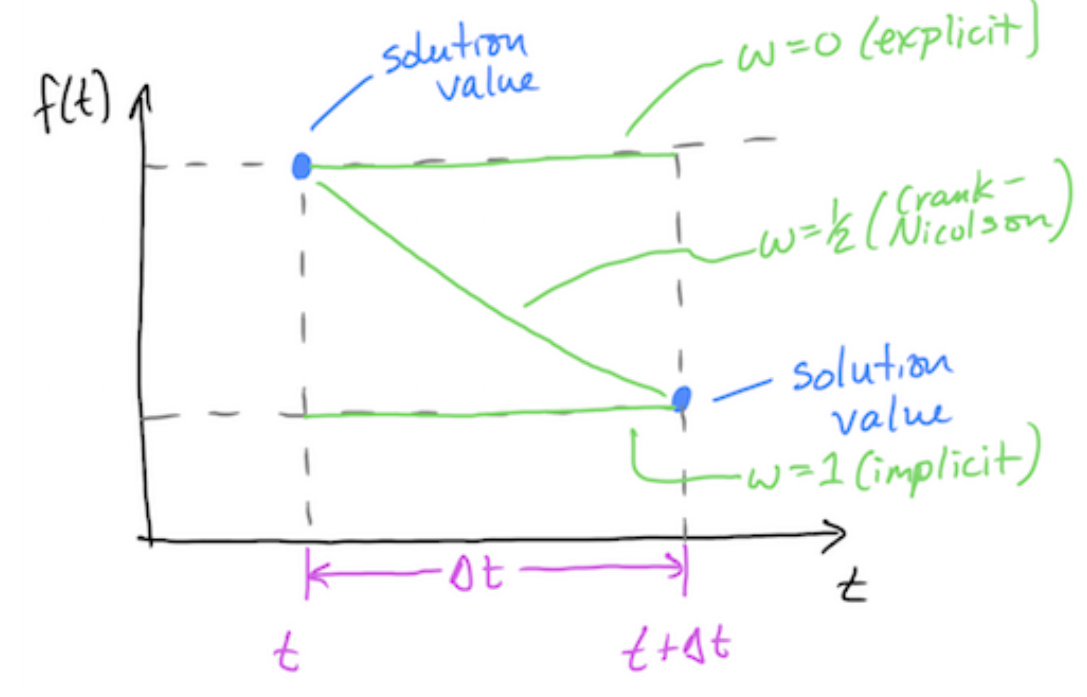
\includegraphics[scale=0.3]{pic/transientHeat_omega.png}
\end{center}
Grouping the time levels together:
\begin{equation}
 \int_{t_0}^{t_1} \int_{V} k \nabla^2 T dt dV = \left[\omega[F_w^d-F_e^d \right ]^{t+\Delta t}\Delta t +
 (1-\omega)\left [F_w^d - F_e^d \right ]^t\Delta t
\end{equation}
Assuming no source term, \(S = 0\), constant properties and divide by \(\Delta t\), our discretized equation becomes
 \begin{equation}
\rho c_p \frac{T_P^{t+\Delta t} - T_P^t}{\Delta t} V_P = \omega \left[F_w^d-F_e^d \right ]^{t+\Delta t} +
  (1-\omega)\left [F_w^d - F_e^d \right ]^t\
 \end{equation}
\textbf{\uline{Note}}
\begin{itemize}
\item fully implicit and fully explicit are \emph{1st order} accurate in time.
\item Crank-Nicolson are \emph{2nd order} accurate in time.
\begin{itemize}
\item but Crank-Nicolson are \emph{less stable}, cause oscillations.
\end{itemize}
\item Generally, explicit solutions do not require the solution of a system of equations. All diffusive fluxes are calculated using solution values from previous timestep
\item Implicit requires solution of a linear system at current time step. The same is true for Crank-Nicolson, or any scheme where \(0<\omega < 1\)
\end{itemize}
\subsection{Analysis of Explicit Scheme}
\label{sec:org576a0c1}
Recall explicit scheme means \(\omega = 0\). Our discretized equation becomes:
\begin{equation}
\rho c_p \frac{T_P ^{t+\Delta t}}{\Delta t} V_P = [F_w^d-F_e^d]^t + \rho c_p \frac{T_P^t}{\Delta t}V_P 
\end{equation}
Recall that the fluxes can be defined as:
\begin{alignat}{2}
F_{e}^d &= - k\frac{T_E-T_P}{\Delta x_{PE}}A_e &&= -D_e(T_E- T_P)\\
F_{w}^d &= - k\frac{T_P-T_W}{\Delta x_{WP}}A_w &&= -D_w(T_P- T_W)\\
D_e &= \frac{kA_e}{\Delta x_{PE}}\\
D_w &= \frac{kA_w}{\Delta x_{WP}}
\end{alignat}
Thus, our explicit formulation becomes:
\begin{equation}
\rho c_p \frac{T_P ^{t+\Delta t}}{\Delta t} V_P = D_eT_E^t + D_wT_W^t + \left ( \frac{\rho c_p V_P}{\Delta t} - D_e - D_w \right)T_P^t 
\end{equation}
To get correct physical influence, the coefficient of \(T_P^t\) must be positive, to ensure \(\uparrow T_P^t\) leads to \(\uparrow T_P^{t+\Delta t}\).
Therefore, our timestep must be selected such that:
\begin{equation*}
\frac{\rho c_p V_P}{\Delta t} \geq D_e + D_w 
\end{equation*}
or
\begin{equation*}
\Delta t \leq \frac{\rho c_p V_P}{D_e + D_w} = \frac{1}{\frac{D_e}{\rho c_p V_P} + \frac{D_w}{\rho c_p V_P} }
\end{equation*}
Simplifying further, we assume \(V_P = A\Delta x\) where \(A\) is the cross-sectional area of the domain at \(P\), and \(\Delta x\) is the grid spacing.
Also assuming \(A_e, A_w \approx A\)
\begin{equation*}
\frac{D_e}{\rho c_p V_P} \approx \frac{\frac{kA_e}{\Delta x}}{\rho c_p A \Delta x} = \frac{k}{\rho c_p}\frac{1}{\Delta x^2} = \frac{\alpha}{\Delta x^2}
\end{equation*}
The quantity \(\frac{\Delta x^2}{\alpha}\) may be interpreted as the timescale associated with conduction through the face.\\
For uniform grid, \(A_e =
   A_w = A\), the timestep restriction is:
\begin{equation}
\Delta t \leq \frac{1}{\frac{\alpha}{\Delta x^2} + \frac{\alpha}{\Delta x^2}} = \frac{\Delta x^2}{2\alpha}
\end{equation}
Note how our timestep is related to the square of the grid size, so the a fine grid will have a very small "\(\Delta x^2\)".
\newpage \noindent
To study this, we consider an iron bar with \(\alpha = 23.1 \times 10^{-6}\) [\(m^2/s\)] at various grid sizes:
\begin{table}[htbp]
\label{tab:orgd03cba0}
\centering
\begin{tabular}{rr}
\hline
GRID SIZE [m] & TIME STEP [sec]\\
\hline
0.01 & 2.1645022\\
0.001 & 0.021645022\\
0.0001 & 2.1645022e-4\\
0.00001 & 2.1645022e-6\\
\hline
\end{tabular}
\end{table}
\begin{center}
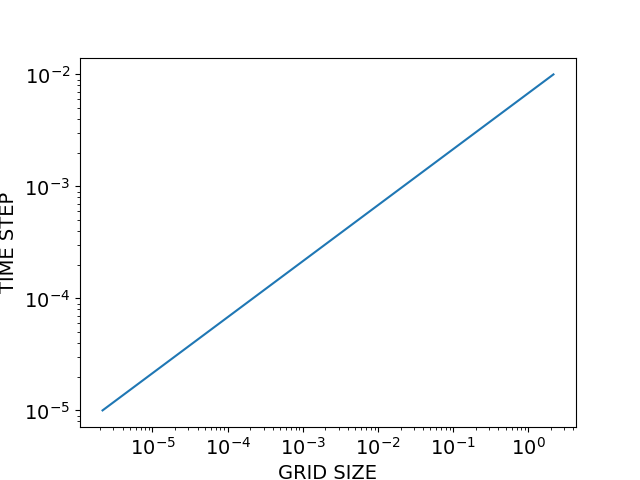
\includegraphics[scale=0.6]{pic/explicit_timestep.png}
\end{center}
We can quickly see how the timestep restriction gets worse with increasing grid refinement. As a result, implicit methods are more commonly used
in practice. Exception would be calculation of turbulent flow using direct numerical simulation (DNS). In this case, explicit method are a good choice
because they are less expensive per timestep, since no linear system must be solved. 
\subsection{Analysis of Fully Implicit Scheme}
\label{sec:org311bbf9}
Setting \(\omega = 1\) for implicit scheme. Our discretized equation becomes:
\begin{equation}
\rho c_p \frac{T_P ^{t+\Delta t}-T_P^t}{\Delta t} V_P = [-D_w(T_P-T_W) + D_e(T_E-T_P)]^{t+\Delta t} 
\end{equation}
Drop the superscript \(t+\Delta t\) and denotes old value as "o", after rearranging, we have:
\begin{equation}
\left ( \frac{\rho c_p V_P}{\Delta t} + D_w + D_e \right)T_P = D_wT_W + D_eT_E + \frac{\rho c_p V_P}{\Delta t}T_P^o
\end{equation}
We can see that none of the coefficients can be come negative when written out this way. Still, we must ensure the timestep is small enough to resolve
all transient phenomena. In contrast to this fully implicit scheme, the \uline{Crank-Nicholson scheme} has no formal restriction on \(\Delta t\), but still
produces \textbf{oscillatory} at large \(\Delta t\). 
\subsection{Derivation of Second Order Implicit Scheme}
\label{sec:org32bea15}
\subsubsection{General idea}
\label{sec:orga4a246d}
We consider integration over a special \textbf{space-time control volume}, with:
\begin{itemize}
\item the time faces being located at \(t-\Delta t/2, t+ \Delta t/2\)
\item the solution values are stored at \$t, t - \(\Delta\) t, t - 2\(\Delta\) t\ldots{}\$.
\end{itemize}
\begin{center}
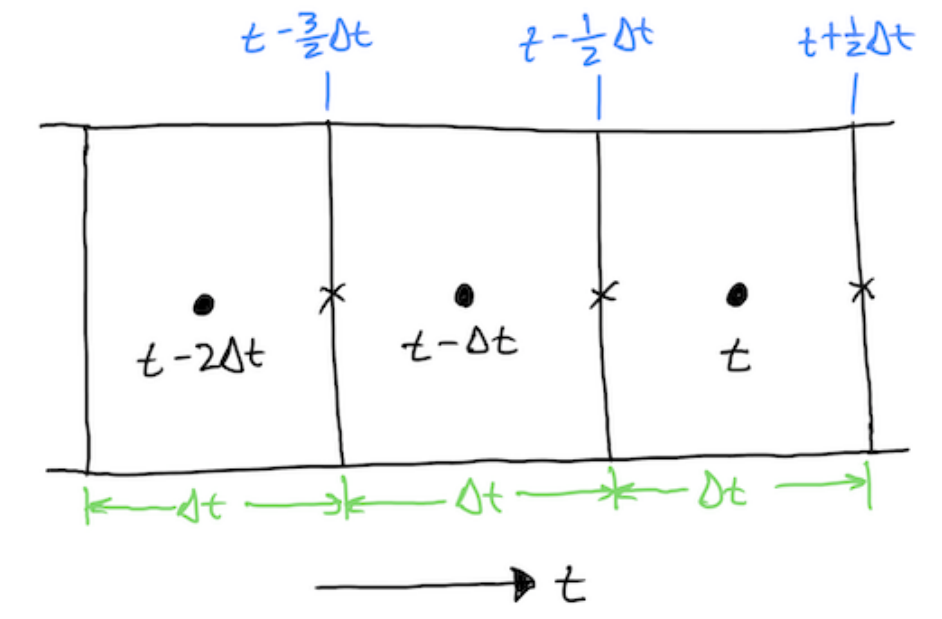
\includegraphics[scale=0.3]{pic/cv_2nd_order_implicit.png}
\end{center}
By using the space-time control volume, the RHS of the discretized equation evaluated at time \(t\), can be considered as a
\uline{representative of the entire timesweep}. The advantages are:
\begin{itemize}
\item we do not need to assume a profile in time, e.g. piecewise constant for fully implicit/explicit, piecewise linear for Crank-Nicholson.
\item no need to store old flux value
\item interpolation depends on the face values:
\begin{itemize}
\item if piecewise constant \(\rightarrow\) 1st order scheme
\item if piecewise linear \(\rightarrow\) 2nd order scheme
\end{itemize}
\end{itemize}
\subsubsection{Derivation}
\label{sec:org883e8a2}
Integrate the governing equation over the space-time control volume 
\begin{equation}
\int_{t-\Delta t/2}^{t+\Delta t/2} \int_{V} \frac{(\partial \rho c_p T)}{\partial t} dt dV =
\int_{t-\Delta t/2}^{t+\Delta t/2} \int_{V} k \nabla^2 T dt dV + \int_{t-\Delta t/2}^{t+\Delta t/2} \int_{V} S dt dV
\end{equation}
Resulting in:
\begin{equation}
(\rho c_p T_p V_p)^{t+\Delta t/2} - (\rho c_p T_p V_p)^{t-\Delta t/2} = [F_w^d-F_e^d]^t \Delta t + S_P^t \Delta t V_P
\end{equation}
Divide by \(\Delta t\), express the diffusive fluxes in terms of \(D_w\) and \(D_e\), dropping superscripts \(t\) for current time:
\begin{equation}
\frac{(\rho c_p T_P V_P)^{t+\Delta t /2 } - (\rho c_p T_P V_P)^{t-\Delta t /2 }  }{\Delta t} = -D_w (T_P-T_W)
+ D_e (T_E - T_P) + S_P V_P
\end{equation}
LHS is known, for RHS \(\rightarrow\) need to specify values for times \$t-\(\Delta\) t/2 and \(t+\Delta t /2\)
\begin{itemize}
\item 1st order time integration scheme
We assume a \textbf{piecewise constant} distribution over each timestep between the face values, resulting in:
\begin{align*}
T_P^{t-\Delta t /2 } &= T_P^{t-\Delta t }\\
T_P^{t+\Delta t /2 } &= T_P^{t}
\end{align*}
\item 2nd order time integration scheme
We assume a \textbf{piecewise linear} distribution over each timestep between the face values, resulting in:
\begin{align*}
T_P^{t-\Delta t /2} &= T_P^{t-\Delta t } + \frac{1}{2}(T_P^{t-\Delta t} - T_P^{t-2\Delta t})\\
T_P^{t+\Delta t /2} &= T_P^{t} + \frac{1}{2}(T_P^{t} - T_P^{t-\Delta t})\\
\end{align*}
This is achieved by doing backward interpolation and then forward interpolation on the face values.
The schematic below shows these interpolations:
\begin{center}
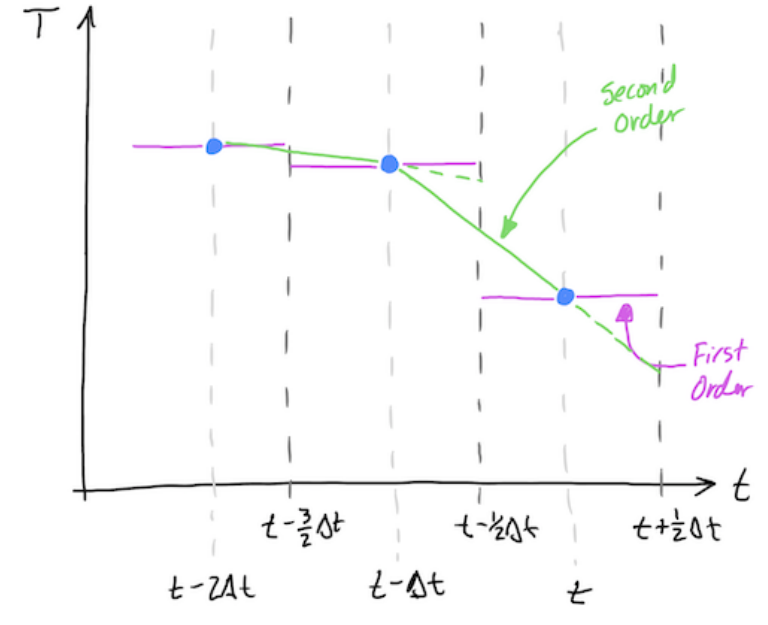
\includegraphics[scale=0.5]{pic/2nd_order_implicit_interpolation.png}
\end{center}
Substituting these relations to the integrated governing equation's LHS:
\begin{itemize}
\item For 1st order scheme:
\begin{equation}
\frac{(\rho c_p T_P V_P)^{t+\Delta t /2} - (\rho c_p T_P V_P)^{t-\Delta t /2 }}{\Delta t} = \rho c_p V_P \frac{T_P - T_P^o}{\Delta t}
\end{equation}
\uline{Note}:
\begin{itemize}
\item the superscript for current time is dropped, and superscript for \(t-\Delta t\) is replaced by \uline{\(o\)} for "old value".
\item also that this is exactly the same as the result for the fully implicit scheme.
\end{itemize}
\item For 2nd order scheme:
\begin{equation*}
\frac{(\rho c_p T_P V_P)^{t+\Delta t /2} - (\rho c_p T_P V_P)^{t-\Delta t /2 }}{\Delta t} =
\rho c_p V_P \frac{T_P + \frac{1}{2}(T_P - T_P^o) - T_P^o - \frac{1}{2}(T_P^o-T_P^{oo})}{\Delta t}
\end{equation*}
or a more simplified version\ldots{}.
\begin{equation}
\frac{(\rho c_p T_P V_P)^{t+\Delta t /2} - (\rho c_p T_P V_P)^{t-\Delta t /2 }}{\Delta t} =
\rho c_p V_P \frac{\frac{3}{2}T_P -2T_P^o + \frac{1}{2}T_P^{oo}}{\Delta t}
\end{equation}
\uline{Note}:
\begin{itemize}
\item superscript \uline{\(oo\)} is used for time value \(t-2\Delta t\).
\item unlike Crank-Nicholson's, flux values at previous timestep \textbf{do not need to be solved}.
Instead, only temperature values at the \textbf{previous two time step} need to be retained.
\end{itemize}
\end{itemize}
\end{itemize}
\subsubsection{Other Transient Discretization Schemes}
\label{sec:orgd033c29}
Some higher order schemes are also used such as:
\begin{itemize}
\item Adams-Bashforth (explicit)
\item Adams-Moulton (implicit)
\item Runge-Kutta (implicit or explicit)
\end{itemize}
\subsubsection{Linearization}
\label{sec:orgcc30f9e}
Recall the cell residual for steady conduction:
\begin{equation*}
r_P = D_w (T_P - T_W) - D_e (T_E - T_P) - S_PV_P
\end{equation*}
where \(D_e = \frac{kA_e}{\Delta x_{PE}}\), and \(D_w = \frac{kA_w}{\Delta x_{WP}}\).
If we apply 1st order implicit to the transient term:
\begin{equation*}
r_P = \rho c_p V_P \frac{T_P-T_P^o}{\Delta t}D_w (T_P - T_W) - D_e (T_E - T_P) - S_PV_P
\end{equation*}
This makes the linearization coefficients to be as follow:
\begin{align*}
a_P &= \frac{\partial r_P}{\partial T_P} = \frac{\rho c_p V_P}{\Delta t} + D_w + D_e - \frac{\partial S_P}{\partial T_P}V_P\\
a_W &= \frac{\partial r_P}{\partial T_W} = -D_w\\
a_E &= \frac{\partial r_P}{\partial T_E} = -D_e  
\end{align*}
Similar to before, we can form an algebraic equation for each control volume like this:
\begin{equation}
a_P\delta T_P + a_W\delta T_W + a_E \delta T_E = -r_P 
\end{equation}
If we apply 2nd order implicit temporal scheme instead, then \(a_P\) term would look like this:
\begin{equation*}
a_P = \frac{\partial r_P}{\partial T_P} = \frac{3}{2}\frac{\rho c_p V_P}{\Delta t} + D_w + D_e - \frac{\partial S_P}{\partial T_P}V_P
\end{equation*}
\end{document}